
%%%%%%%%%%%%%%%%%%%%%%%%%%%%%%%%%%%%%%%%%%%%%%%%%%
\begin{frame}[fragile]{Our Starting Point}
\begin{itemize}
\item Business Software
\item Very poor code quality
\item Planned changes for a module:
\begin{itemize}
\item Bugfixing
\item new features
\item better tests
\end{itemize}
\end{itemize}

$\Rightarrow$ A restructuring was required
\end{frame}

%%%%%%%%%%%%%%%%%%%%%%%%%%%%%%%%%%%%%%%%%%%%%%%%%%
\begin{frame}[fragile]{The Domain}
\begin{itemize}
\item Financial mathematical software
\end{itemize}

\begin{itemize}
\item Calculate for a bank account for each month:
\begin{itemize}
\item Balance at the last day of the month (ultimo)
\item Average balance of the month
\end{itemize}
\end{itemize}

\end{frame}


%%%%%%%%%%%%%%%%%%%%%%%%%%%%%%%%%%%%%%%%%%%%%%%%%%
\begin{frame}[fragile]{Problems of the Existing Code Structure}
\begin{itemize}
\item Code writes values into separate data objects (\glqq Push\grqq{})
\item Multiple writing operations for one value
\item Parts of  the code access previously written values
\item Code is driven by the view from the inside: What do I need to do in summary to be able to deliver a set of result values?
\end{itemize}
\end{frame}

%%%%%%%%%%%%%%%%%%%%%%%%%%%%%%%%%%%%%%%%%%%%%%%%%%
\begin{frame}[fragile]{Problems of the Existing Code Structure}
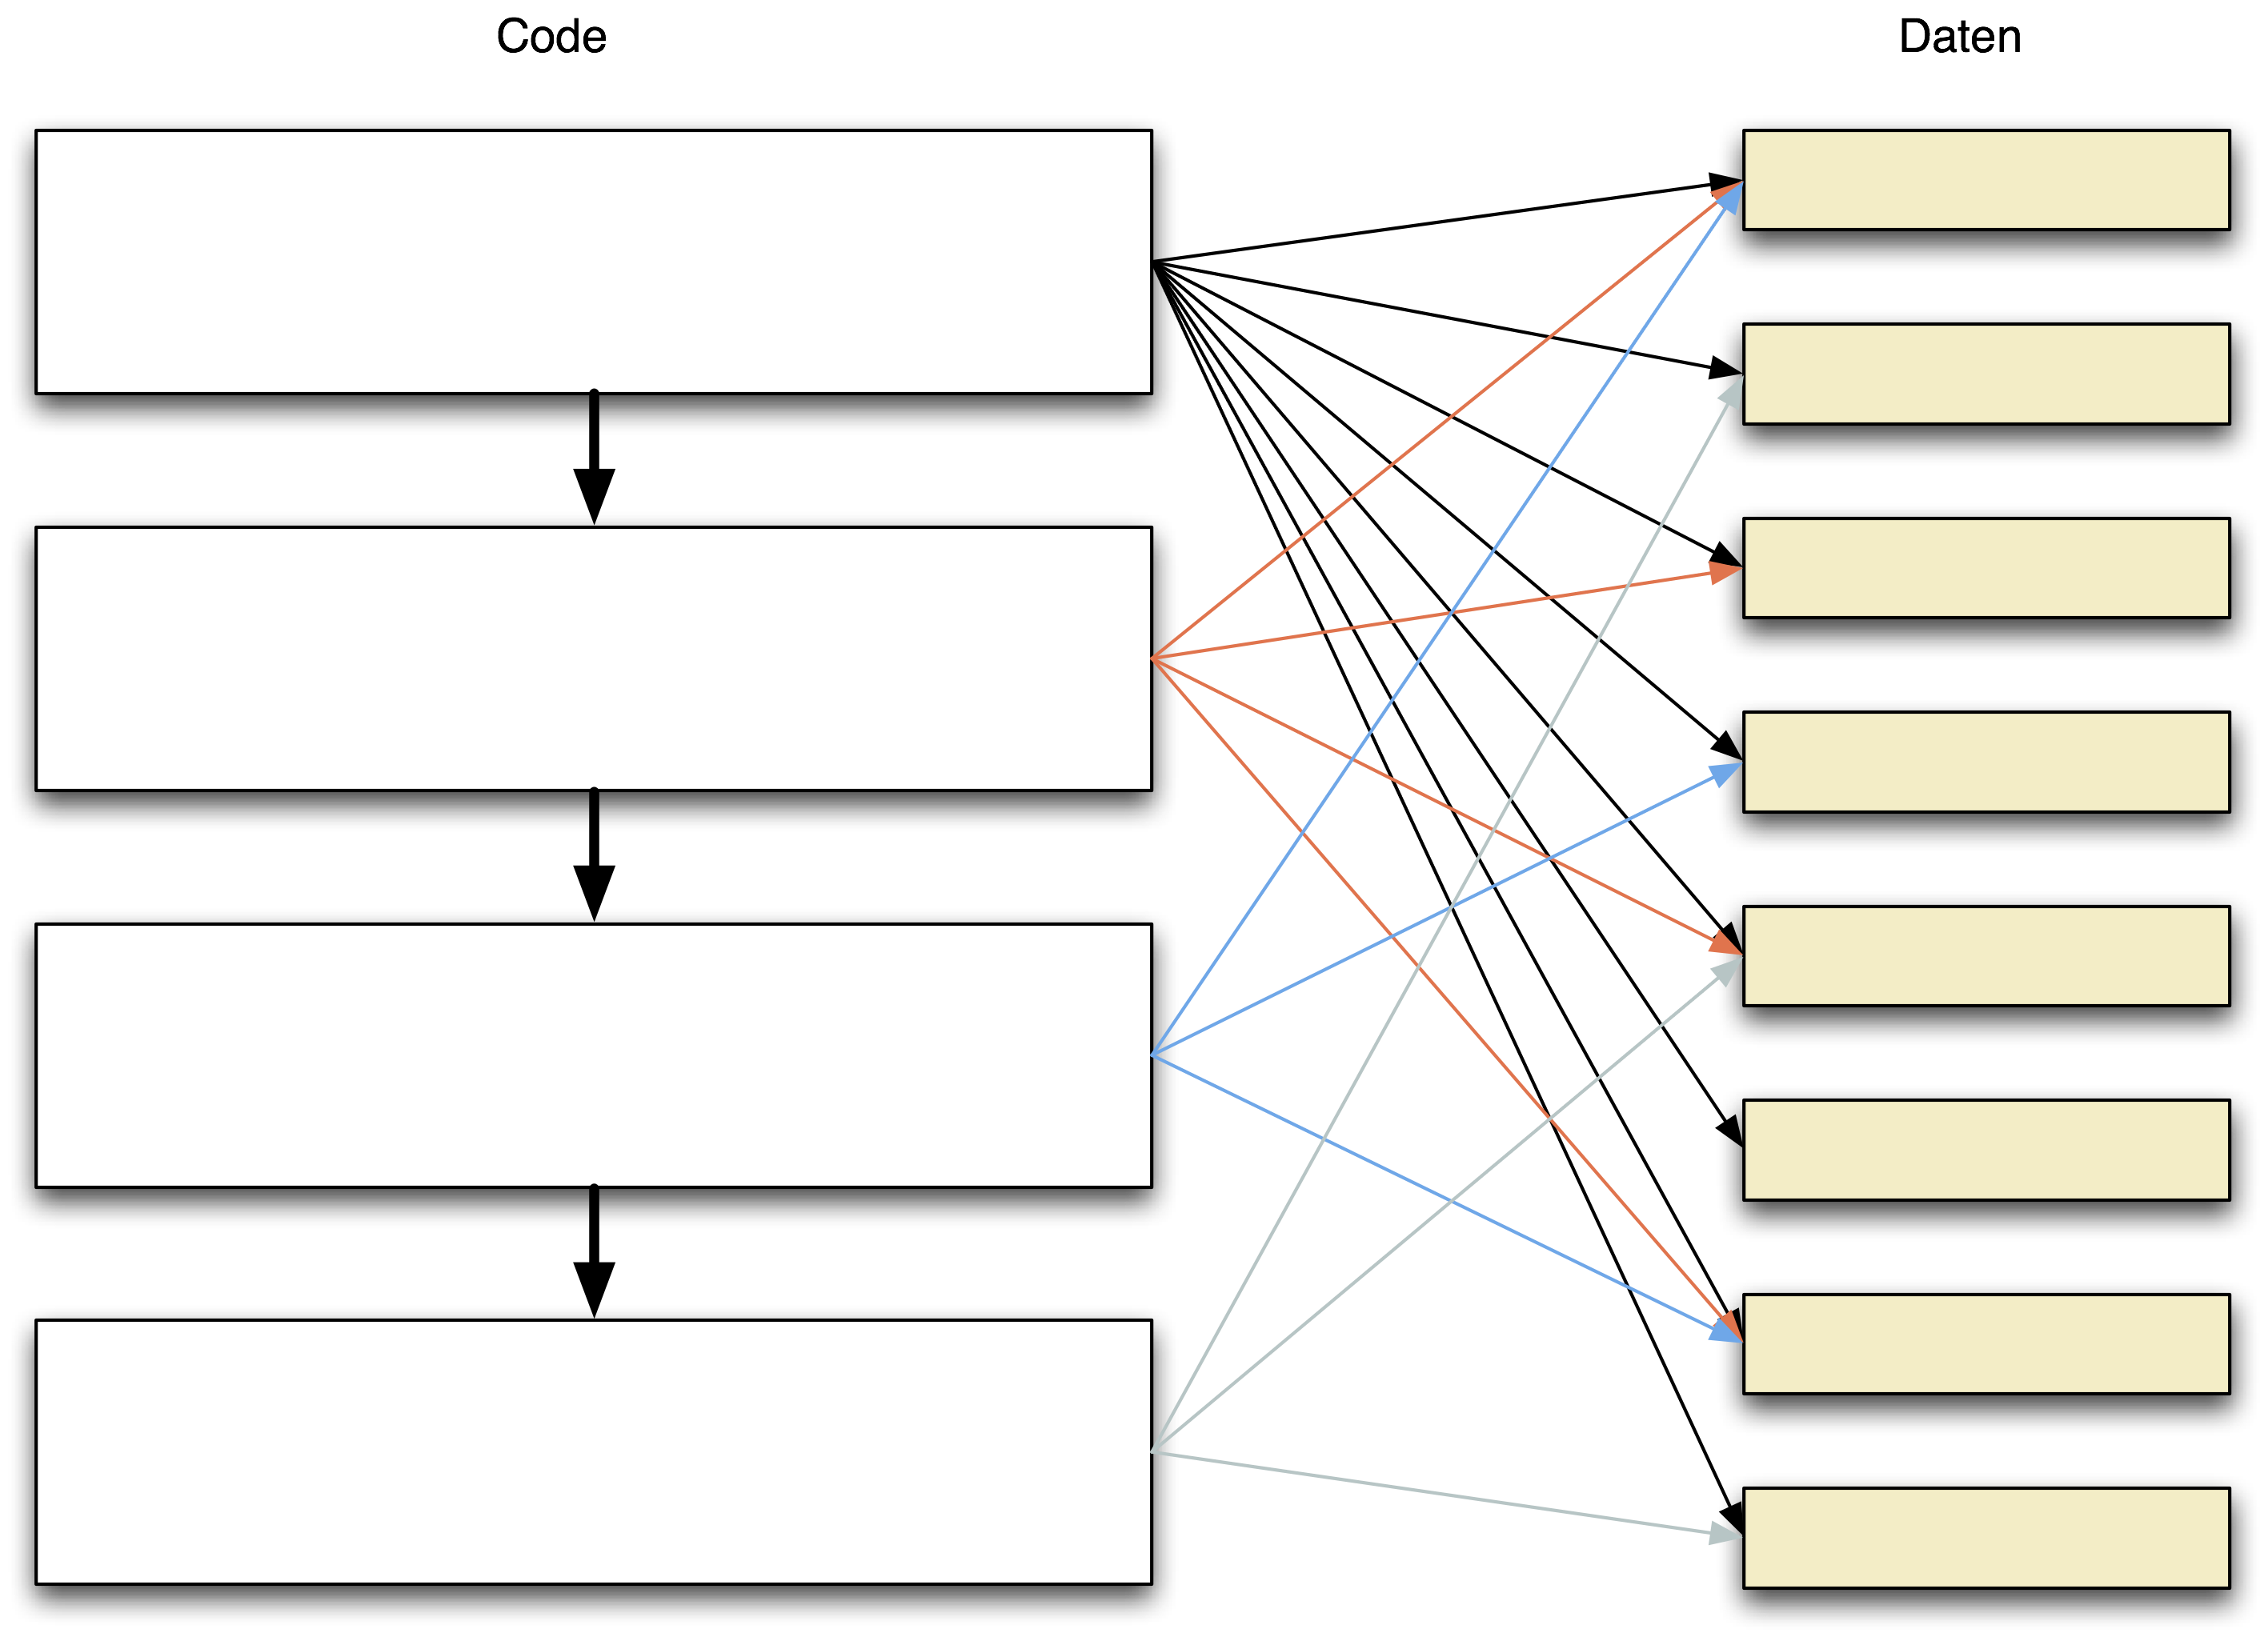
\includegraphics[width=.85 \paperwidth]{Codestruktur.png}
\end{frame}

%%%%%%%%%%%%%%%%%%%%%%%%%%%%%%%%%%%%%%%%%%%%%%%%%%
\begin{frame}[fragile]{Goal}
\begin{itemize}
\item Structure:
\begin{itemize}
\item Code mirrors the business logic
\end{itemize}
\end{itemize}

\begin{itemize}
\item View from the outside, driven by the expected results:
\begin{itemize}
\item Which values do I need?
\item How is each value calculated?
\item Which categories of results exist? Similarities, differences?
\end{itemize}
\end{itemize}
\end{frame}

%%%%%%%%%%%%%%%%%%%%%%%%%%%%%%%%%%%%%%%%%%%%%%%%%%
\begin{frame}[fragile]{Goal}
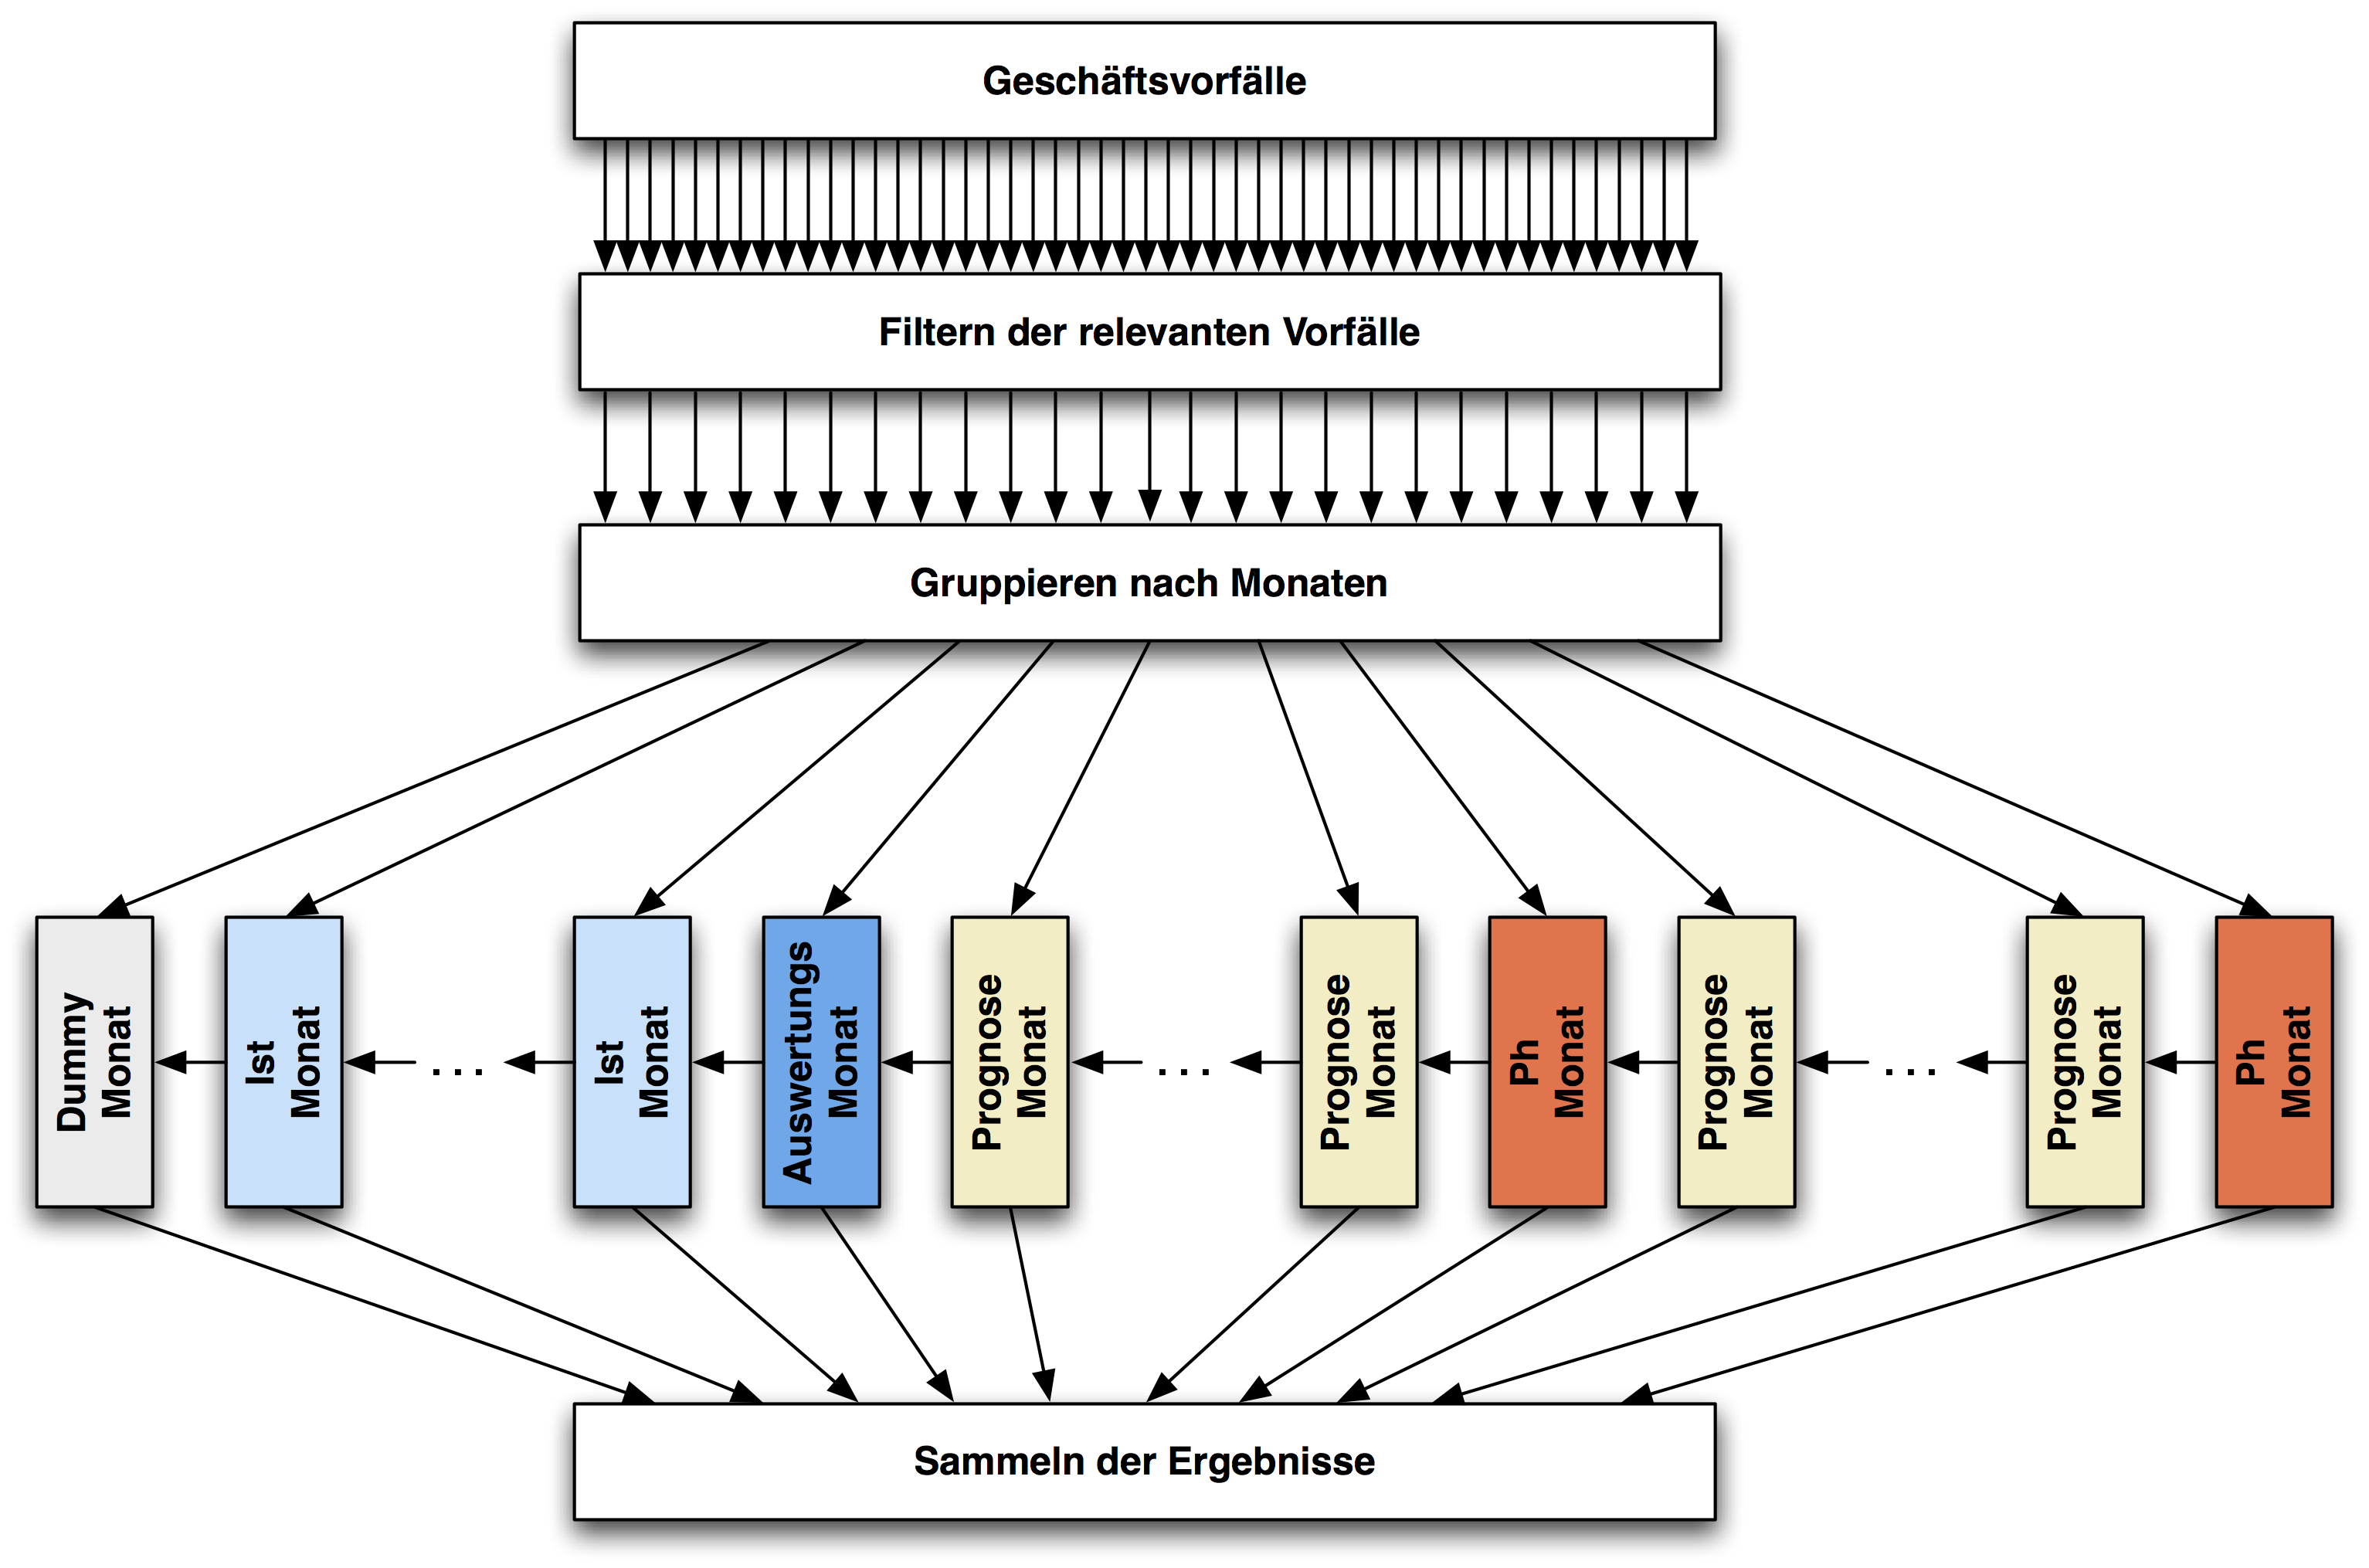
\includegraphics[width=.85 \paperwidth]{DynamischFein.jpg}
\end{frame}


%%%%%%%%%%%%%%%%%%%%%%%%%%%%%%%%%%%%%%%%%%%%%%%%%%
\begin{frame}[fragile]{Good Approach}
\begin{itemize}
\item Feature-toggle to compare the old and the new version
\begin{itemize}
\item Identification or creation of a minimal entry point to the restructured area
\item The API of this entry point must remain unchanged
\end{itemize}
\end{itemize}

\begin{itemize}
\item Important aspects of the restructuring:
\begin{itemize}
\item Driven by business logic
\item Purely structural
\end{itemize}
\end{itemize}

\begin{itemize}
\item Technical goal:
\begin{itemize}
\item Separation of Concerns
\item On-demand-calculation of all values (\glqq Pull\grqq{})
\item Bonus: Value caching via lazy initialization
\end{itemize}

\end{itemize}
\end{frame}

%%%%%%%%%%%%%%%%%%%%%%%%%%%%%%%%%%%%%%%%%%%%%%%%%%
\begin{frame}[fragile]{Important!}
\begin{itemize}
\item If in doubt, the existing code shows the correct behaviour!

\item Do not change the logic while restructuring!

\item Explicit approval of the restructuring
\begin{itemize}
\item It must show identical behaviour (tests, bugs, features)
\end{itemize}

\end{itemize}
\end{frame}




%%%%%%%%%%%%%%%%%%%%%%%%%%%%%%%%%%%%%%%%%%%%%%%%%%
\begin{frame}[fragile]{Workshop}

\begin{center}
{\huge Workshop}
\end{center}
\end{frame}

%%%%%%%%%%%%%%%%%%%%%%%%%%%%%%%%%%%%%%%%%%%%%%%%%%
\begin{frame}[fragile]{Balance}
\begin{center}
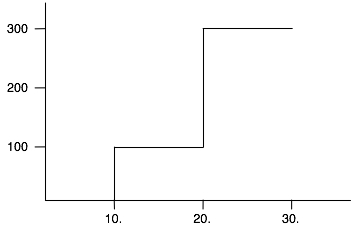
\includegraphics[width=.85 \paperwidth]{../workshopMaterial/balance.jpg}
\end{center}
\end{frame}

%%%%%%%%%%%%%%%%%%%%%%%%%%%%%%%%%%%%%%%%%%%%%%%%%%
\begin{frame}[fragile]{Initial Average}
\begin{center}
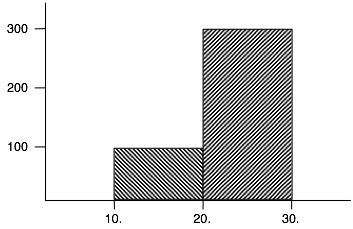
\includegraphics[width=.85 \paperwidth]{../workshopMaterial/initialAverage.jpg}
\end{center}
\end{frame}

%%%%%%%%%%%%%%%%%%%%%%%%%%%%%%%%%%%%%%%%%%%%%%%%%%
\begin{frame}[fragile]{Final Average}
\begin{center}
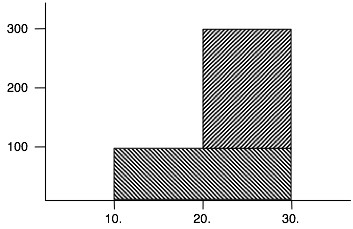
\includegraphics[width=.85 \paperwidth]{../workshopMaterial/finalAverage.jpg}
\end{center}
\end{frame}

%%%%%%%%%%%%%%%%%%%%%%%%%%%%%%%%%%%%%%%%%%%%%%%%%%

%%%%%%%%%%%%%%%%%%%%%%%%%%%%%%%%%%%%%%%%%%%%%%%%%%
{
\usebackgroundtemplate{
\includegraphics[width=\paperwidth,height=\paperheight]{background-slide.png}}
\begin{frame}{Thank you!}

        Code \& slides at GitHub:
        \begin{center}
                \url{https://github.com/NicoleRauch/RefactoringLegacyCode}
        \end{center}

        \begin{block}{Andreas Leidig}
        \begin{description}[Twitterxx]
                \item[E-Mail]  \href{mailto:andreas.leidig@msg-gillardon.de}{\texttt{andreas.leidig@msg-gillardon.de}}
                \item[Twitter] \href{http://twitter.com/leiderleider}{\texttt{@leiderleider}}
        \end{description}
        \end{block}

        \begin{block}{Nicole Rauch}
        \begin{description}[Twitterxx]
                \item[E-Mail]  \href{mailto:nicole.rauch@msg-gillardon.de}{\texttt{nicole.rauch@msg-gillardon.de}}
                \item[Twitter] \href{http://twitter.com/NicoleRauch}{\texttt{@NicoleRauch}}
        \end{description}
        \end{block}
\end{frame}
}
